\documentclass{beamer}	
\usecolortheme{wolverine}

\setbeamertemplate{caption}{\raggedright\insertcaption\par}

\usepackage{tabularx}
\usepackage{booktabs}
\usepackage{multirow}
\newcolumntype{C}{>{\centering\arraybackslash}X}
\usepackage{proof}
\usepackage{amsmath}
\usepackage{wasysym}
\usepackage{tikz}
\usetikzlibrary{arrows.meta,positioning,matrix}
\usepackage{qtree}

\newcommand{\term}[1]{\texttt{#1}}
\newcommand{\li}{\!\multimap\!}
\newcommand{\lotimes}{\!\otimes\!}
\newcommand{\loplus}{\!\oplus\!}
\newcommand{\lin}[1]{\langle#1\rangle}
\newcommand{\lint}[1]{[#1]}

\title{Lambek Calculus}
\author{K. Kogkalidis}
\institute{Logic \& Language 2020}

\begin{document}
\date{}
\maketitle

%\begin{frame}{IIL$~_{\li}$ w/o Commutativity}
%	\small
%	Dropping \alert{Exchange}, the implication rules:
%	\[
%		\infer[]{A\li B, A \vdash B}{
%			{A\li B \vdash A\li B}
%			&
%			{A \vdash A}
%		}
%		\quad\quad
%		\infer[\li I]{\Gamma \vdash A\li B}{
%			\Gamma, A \vdash B
%		}
%	\]
%	do not suffice 
%
%\end{frame}

\begin{frame}{Categorial Grammars: History}
	\small
	\begin{minipage}[t]{0.4\textwidth}
		\begin{minipage}[t]{1\textwidth}
		\begin{figure}
		\includegraphics[width=0.5\textwidth]{Adjukiewicz}
		\caption{Kazimierz Ajdukiewicz}
		\end{figure}
		\end{minipage}
		\vfill
		\begin{minipage}[t]{1\textwidth}
		\begin{figure}
		\includegraphics[width=0.5\textwidth]{BarHillel}
		\caption{Yehoshua Bar-Hillel}
		\end{figure}	
		\end{minipage}	
	\end{minipage}%
	\begin{minipage}[t]{0.6\textwidth}
		\begin{block}{AB Grammars}
		An AB Grammar is a tuple $\left( \Sigma, \mathcal{A}, S, L \right)$
		\begin{itemize}
		\item[$\Sigma$] a finite set of symbols
		\item[$\mathcal{A}$] a finite set of primitives, deriving:
		\[
			\mathcal{T}_\mathcal{A} := \mathcal{A} \ | \  \mathcal{T}_\mathcal{A}/\mathcal{T}_\mathcal{A} \ | \ \mathcal{T}_\mathcal{A} \backslash\mathcal{T}_\mathcal{A}
		\]
		\item[$S$] a distinguished type, $S \in \mathcal{T}_\mathcal{A}$
		\item[$L$] a mapping $\Sigma \to \mathcal{T}_\mathcal{A}$
		\end{itemize}		
		\end{block}	
		\vfill
		
		\begin{block}{Inference Rules}
		\begin{itemize}
			\item[] $X \longleftarrow X/Y, Y$
			\item[] $X \longleftarrow Y, Y\backslash X$
		\end{itemize}
		\end{block}
	\end{minipage}
\end{frame}

\begin{frame}{AB Grammars \& Constituency Parsing}
	\small
	\begin{minipage}{0.4\textwidth}
	Consider a grammar where
	\begin{itemize}
		\item[$\mathcal{A}$] := $\{S, N, NP \}$
		\item[$\Sigma$] a (simple) lexicon of english
		\item[$L$] a mapping from: 
			\item[] {\footnotesize common nouns to $n$}
			\item[] {\footnotesize proper nouns to $np$}
			\item[] \footnotesize{ determiners to $np/n$}
			\item[] {\footnotesize adjectives to $n/n$}
			\item[] {\footnotesize intrasitive verbs to $np\backslash s$} 
			\item[] {\footnotesize transitive verbs to $(np\backslash s)/np$}
			\item[] \dots
	\end{itemize}	
	\end{minipage}%
	\pause
	\begin{minipage}{0.6\textwidth}
	{\footnotesize
	\Tree
	[.$s$
		[.$np$
			Pietr
		]
		[.${np\backslash s}$
			[.$(np\backslash s)/np$
				wrote
			]
			[.$np$
				[.$np/n$
					an
				]
				[.$n$
					[.$n/n$
						important
					]
					[.$n$
						book
					]
				]
			]
		]
	]
	}	
	\centering
	Pietr (wrote (an (important book)))
	\end{minipage}
\end{frame}

\begin{frame}{Refinement: Lambek Calculus L}
	\small
	\begin{minipage}[t]{0.3\textwidth}
		\begin{figure}
		\includegraphics[width=0.7\textwidth]{Lambek}
		\caption{Joachim Lambek}
		\end{figure}	
	\end{minipage}%
	\begin{minipage}[t]{0.65\textwidth}
	\alert{The Mathematics of Sentence Structure (1958)}:
		\[
			\mathcal{T}_{\mathcal{A}} := \mathcal{A} \ | \ \mathcal{T}_\mathcal{A}/\mathcal{T}_\mathcal{A} \ | \ \mathcal{T}_\mathcal{A}\backslash \mathcal{T}_\mathcal{A} \ | \ \mathcal{T}_\mathcal{A}\otimes \mathcal{T}_\mathcal{A}
		\]
		\vspace{-20pt}
		\begin{itemize}
			\item[$/$] 'right' division (\textit{over})
			\item[$\backslash$] 'left' division (\textit{under})
			\item[$\otimes$] concatenation (\textit{with})
		\end{itemize}
	\end{minipage}
	\vfill
	\pause
	
	$\rightsquigarrow$ \alert{ILL${}_{\li}$ without Exchange}:
	\[
	\begin{array}{cc}
		\vcenter{\infer[/ E]{\Gamma, \Delta \vdash B}{\Gamma \vdash B/A & \Delta \vdash A}}
		&
		\vspace{5pt}
		\vcenter{\infer[/ I]{\Gamma \vdash B/A}{\Gamma, A \vdash B}} \\		\vcenter{\infer[\backslash E]{\Gamma, \Delta \vdash B}{\Gamma \vdash A & \Delta \vdash A\backslash B}}
		\vspace{5pt}
		&
		\vcenter{\infer[\backslash I]{\Gamma \vdash A\backslash B}{A, \Gamma \vdash B}} \\
		\vcenter{\infer[\otimes E]{\Delta, \Gamma, \Theta \vdash C}{
			\Gamma \vdash A\otimes B
			&
			\Delta, A, B, \Theta \vdash C
		}}
		&
		\vcenter{\infer[\otimes I]{\Gamma, \Delta \vdash A\otimes B}{
			\Gamma \vdash A 
			&
			\Delta \vdash B
			}} \\
	\end{array}
	\]
\end{frame}

\begin{frame}{Lambek Calculus L}
	\small
	\alert{The Lambek Calculus L}\\
	\begin{itemize}
	\item is the grammar of \alert{strings}, being order-sensitive
	\item is a substructural logic coinciding with the non-commutative fragment of multiplicative intuitionistic linear logic $\text{ILL}_{\otimes, /, \backslash}$
	\item[] $\implies$ assumptions of L are no longer multisets, but \alert{sequences}
	\item has equal generative capacity to AB- and CF-grammars
	\end{itemize}

\end{frame}

\begin{frame}{Further Refinement: NL}
	\small
	The $,$ of L assumptions still hides an implicit structural rule:
	\pause
	associativity
	\vfill

	\alert{On the Calculus of Syntactic Types (1961)}:\\
	
	Assumptions are now bracketed structures $\mathcal{S} := \mathcal{T}_\mathcal{A} \ | \ (\mathcal{S}, \mathcal{S})$
	\pause
		
	\[
	\begin{array}{cc}
		\vcenter{\infer[/ E]{(\Gamma, \Delta) \vdash B}{\Gamma \vdash B/A & \Delta \vdash A}}
		&
		\vspace{5pt}
		\vcenter{\infer[/ I]{\Gamma \vdash B/A}{(\Gamma, A) \vdash B}} \\		\vcenter{\infer[\backslash E]{(\Gamma, \Delta) \vdash B}{\Gamma \vdash A & \Delta \vdash A\backslash B}}
		\vspace{5pt}
		&
		\vcenter{\infer[\backslash I]{\Gamma \vdash A\backslash B}{(A, \Gamma) \vdash B}} \\
		\vcenter{\infer[\otimes E]{\Delta[\Gamma] \vdash C}{
			\Gamma \vdash A\otimes B
			&
			\Delta[(A, B)] \vdash C
		}}
		&
		\vcenter{\infer[\otimes I]{(\Gamma, \Delta) \vdash A\otimes B}{
			\Gamma \vdash A 
			&
			\Delta \vdash B
			}} \\
	\end{array}
	\]
	\begin{flushright}
		where $\Gamma[\Delta]$: $\Delta$ a sub-structure of $\Gamma$	
	\end{flushright}
	
	
	from NL one can recover L via explicit associativity:
	\[
		\infer[A]{\Gamma[((\Delta, \Theta), \Phi)] \vdash C}{
		\Gamma[(\Delta, (\Theta, \Phi))] \vdash C
		}
	\]
	\end{frame}

\begin{frame}{Non-Associative Lambek Calculus NL}
	\small
	\alert{The N/A Lambek Calculus NL}\\
	\begin{itemize}
	\item is the grammar of \alert{trees}, being order- and constituency-sensistive
	\item is a substructural logic coinciding with the non-commutative non-associative fragment of $\text{ILL}_{\otimes, /, \backslash}$
	\item[] $\implies$ assumptions of NL are no longer sequences, but \alert{binary trees}
	\end{itemize}
\end{frame}

\begin{frame}{Example: L vs NL}
	\small
	\alert{
	\[
		B/C \vdash (A/B) \backslash (A/C)
	\]
	}
	
	\alt<6->{Derivation in NL}{Derivation in L}

	\alt<6->{	
	\[
	\infer[\visible<7->{\backslash I}]{{B/C \vdash (A/B) \backslash (A/C)}}{
		\visible<7->{
			\infer[\visible<8->{/ I}]{(A/B, B/C) \vdash A/C}{
			\visible<8->{
				\infer[\visible<9->{\textcolor{red}{A}}]{((A/B, B/C), C) \vdash A}{
				\visible<9->{
					\infer[]{(A/B, (B/C, C)) \vdash C}{\dots}
				}}
			}}
		}}
	\]
	}{
		\[
		\infer[\visible<2->{\backslash I}]{{B/C \vdash (A/B) \backslash (A/C)}}{
		\visible<2->{
			\infer[\visible<3->{/ I}]{A/B, B/C \vdash A/C}{
			\visible<3->{
				\infer[\visible<4->{/E}]{A/B, B/C, C \vdash A}{
				\visible<4->{
					\infer[Ax]{A/B \vdash A/B}{}
					&
					\infer[\visible<5->{/ E}]{B/C, C \vdash B}{
					\visible<5->{
						\infer[Ax]{B/C \vdash B/C}{}
						&
						\infer[Ax]{C \vdash C}{}
					}}
				}}
			}}
		}}
	\]
	}
\end{frame}

\begin{frame}{Parsing $\equiv$ Deduction}
	\small
	\begin{block}{Parsing as Deduction}
		For categorial grammars, syntactic parsing becomes equated with a logical deduction process, proving the well-formedness of a sentence and finding its structure
	\end{block}
	
	\[
		\infer[\backslash E]{\text{(Pietr $\cdot$ (wrote $\cdot$ (an $\cdot$ (important $\cdot$ book))))} \vdash s}{
			\infer[]{\raisebox{0pt}[7pt]{np}}{\text{Pietr}}
			&
			\infer[/E]{\text{(wrote $\cdot$ (an $\cdot$ (important $\cdot$ book)))} \vdash np\backslash s}{
				\infer[]{(np\backslash s)/s}{\text{wrote}}
				&
				\infer[/E]{\text{(an $\cdot$ (important $\cdot$ book))} \vdash np}{
					\infer[]{np/ n}{\text{an}}
					&
					\infer[/ E]{\text{(important $\cdot$ book)} \vdash n}{
						\infer[]{\raisebox{0pt}[6pt]{n/n}}{\text{important}}
						&
						\infer[]{\raisebox{0pt}[6pt]{n}}{\text{book}}
					}
				}
			}
		}
	\]
\end{frame}

\begin{frame}{Ambiguity}
	\small
	\alt<2->{
	Reading 2:
	\[
		\infer[]{\text{(I $\cdot$ ((saw  $\cdot$ (the  $\cdot$ man)) $\cdot$ (with $\cdot$ (the $\cdot$ binoculars)))}\vdash s}{
		?}
	\]
	\visible<3->{
	Need an alternative type for ``with"
	\begin{itemize}
		\item with (producing noun modifier): $(n \backslash n)/np$
		\item with (producing verb-phrase modifier): 	$((np\backslash s)\backslash (np\backslash s))/np$
	\end{itemize}\vfill
	
	\visible<4->{
	Syntactic/structural ambiguity becomes \alert{lexical ambiguity}
	
	
	contrapose: $VP\to VP\ PP$ vs. $N \to N \ PP$	
	
	\begin{flushright}
		lexicaly ambiguous types can be treated with the \alert{$\&$} connective	
	\end{flushright}
	
	}
	{}
	}{}
	}{
	Reading 1:
	\[
		\infer[]{\text{(I $\cdot$ (saw $\cdot$ (the $\cdot$ (man $\cdot$ (with $\cdot$ (the $\cdot$ binoculars))))))} \vdash s}{
			\infer[]{\raisebox{0pt}[6pt]{np}}{\text{I}}
			&
			\infer[]{\raisebox{0pt}[6pt]{$\text{saw $\cdot$ (the $\cdot$ (man $\cdot$ (with $\cdot$ (the $\cdot$ binoculars)))))} \vdash np\backslash s $}}{
				\infer[]{\raisebox{0pt}[6pt]{$(np\backslash s)/s$}}{\text{saw}}
				&
				\infer[]{\raisebox{0pt}[6pt]{$\text{(the $\cdot$ (man $\cdot$ (with $\cdot$ (the $\cdot$ binoculars))))} \vdash np$}}{
					\infer[]{\raisebox{0pt}[6pt]{$\text{np/n}$}}{\text{the}}
					&
					\infer[]{\raisebox{0pt}[6pt]{$\text{(man $\cdot$ (with $\cdot$ (the $\cdot$ binoculars)))} \vdash n$}}{
						\infer[]{\raisebox{0pt}[6pt]{$n$}}{\text{man}}
						&
						\infer[]{\raisebox{0pt}[6pt]{$\text{(with $\cdot$ (the $\cdot$ binoculars))} \vdash n\backslash n$}}{
							\infer[]{\raisebox{0pt}[6pt]{$(n\backslash n)/np$}}{\text{with}}
							&
							\infer[]{\raisebox{0pt}[6pt]{$\text{(the $\cdot$ binoculars)} \vdash np$}}{
								\infer[]{\raisebox{0pt}[6pt]{$np/n$}}{\text{the}}
								&
								\infer[]{\raisebox{0pt}[6pt]{$n$}}{\text{binoculars}}
							}
						}
					}
				}
			}
		}
	\]
	}
\end{frame}

\begin{frame}[fragile]{The Full Substructural Picture}
	\centering
	\begin{minipage}{0.5\textwidth}
	\begin{figure}
	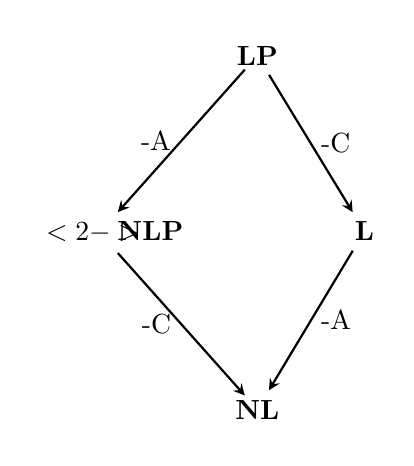
\begin{tikzpicture}
	  \matrix (m) [matrix of math nodes, row sep=5em, column sep=3em]{
		    & \makebox[2pt]{\textbf{LP}} &  \\
		    {\visible<2->{\makebox[2pt]{\textbf{NLP}}}} &  & \makebox[2pt]{\textbf{L}}\\
		     & \makebox[2pt]{\textbf{NL}} & \\};
	\path[-stealth,thick]
	    (m-1-2) edge node[above,right] {-C} (m-2-3)
	    (m-2-3) edge node[above, right] {-A} (m-3-2);
	    \visible<2-> 
	    {\path[-stealth,thick]
	    (m-1-2) edge node[above, left] {-A} (m-2-1)
	    (m-2-1) edge node[above, left] {-C} (m-3-2);
	    }
	\end{tikzpicture}
	\end{figure}
	\end{minipage}%
	\begin{minipage}{0.5\textwidth}
	\small
	\begin{tabularx}{0.95\textwidth}{@{}lccc@{}}
	logic & struct & assoc & commut \\
	\toprule
	LP & multiset & \checkmark & \checkmark \\
	L & string & \checkmark & - \\
	NL & tree & - & - \\
	\visible<2->{NLP & mobile & - & \checkmark}
	\end{tabularx}
	\end{minipage}
\end{frame}

\begin{frame}{Comparison with CFGs}

\begin{itemize}
	\item More ``formal" \\
	\small{The Lambek Calculus defines a substructural logic and an algebra.}
	\item More general \\ 
	\small{Rule size constant with vocabulary size. Lexicalization happens on the lexicon, assigning a type to each ``type'' of word.}
	\item Natural syntax-semantics interface \\ 
	Connection to I(L)L allow easy translation from syntactic to semantic calculus (tbd \dots)
\end{itemize}

\end{frame}

\end{document}